\documentclass[1p]{elsarticle_modified}
%\bibliographystyle{elsarticle-num}

%\usepackage[colorlinks]{hyperref}
%\usepackage{abbrmath_seonhwa} %\Abb, \Ascr, \Acal ,\Abf, \Afrak
\usepackage{amsfonts}
\usepackage{amssymb}
\usepackage{amsmath}
\usepackage{amsthm}
\usepackage{scalefnt}
\usepackage{amsbsy}
\usepackage{kotex}
\usepackage{caption}
\usepackage{subfig}
\usepackage{color}
\usepackage{graphicx}
\usepackage{xcolor} %% white, black, red, green, blue, cyan, magenta, yellow
\usepackage{float}
\usepackage{setspace}
\usepackage{hyperref}

\usepackage{tikz}
\usetikzlibrary{arrows}

\usepackage{multirow}
\usepackage{array} % fixed length table
\usepackage{hhline}

%%%%%%%%%%%%%%%%%%%%%
\makeatletter
\renewcommand*\env@matrix[1][\arraystretch]{%
	\edef\arraystretch{#1}%
	\hskip -\arraycolsep
	\let\@ifnextchar\new@ifnextchar
	\array{*\c@MaxMatrixCols c}}
\makeatother %https://tex.stackexchange.com/questions/14071/how-can-i-increase-the-line-spacing-in-a-matrix
%%%%%%%%%%%%%%%

\usepackage[normalem]{ulem}

\newcommand{\msout}[1]{\ifmmode\text{\sout{\ensuremath{#1}}}\else\sout{#1}\fi}
%SOURCE: \msout is \stkout macro in https://tex.stackexchange.com/questions/20609/strikeout-in-math-mode

\newcommand{\cancel}[1]{
	\ifmmode
	{\color{red}\msout{#1}}
	\else
	{\color{red}\sout{#1}}
	\fi
}

\newcommand{\add}[1]{
	{\color{blue}\uwave{#1}}
}

\newcommand{\replace}[2]{
	\ifmmode
	{\color{red}\msout{#1}}{\color{blue}\uwave{#2}}
	\else
	{\color{red}\sout{#1}}{\color{blue}\uwave{#2}}
	\fi
}

\newcommand{\Sol}{\mathcal{S}} %segment
\newcommand{\D}{D} %diagram
\newcommand{\A}{\mathcal{A}} %arc


%%%%%%%%%%%%%%%%%%%%%%%%%%%%%5 test

\def\sl{\operatorname{\textup{SL}}(2,\Cbb)}
\def\psl{\operatorname{\textup{PSL}}(2,\Cbb)}
\def\quan{\mkern 1mu \triangleright \mkern 1mu}

\theoremstyle{definition}
\newtheorem{thm}{Theorem}[section]
\newtheorem{prop}[thm]{Proposition}
\newtheorem{lem}[thm]{Lemma}
\newtheorem{ques}[thm]{Question}
\newtheorem{cor}[thm]{Corollary}
\newtheorem{defn}[thm]{Definition}
\newtheorem{exam}[thm]{Example}
\newtheorem{rmk}[thm]{Remark}
\newtheorem{alg}[thm]{Algorithm}

\newcommand{\I}{\sqrt{-1}}
\begin{document}

%\begin{frontmatter}
%
%\title{Boundary parabolic representations of knots up to 8 crossings}
%
%%% Group authors per affiliation:
%\author{Yunhi Cho} 
%\address{Department of Mathematics, University of Seoul, Seoul, Korea}
%\ead{yhcho@uos.ac.kr}
%
%
%\author{Seonhwa Kim} %\fnref{s_kim}}
%\address{Center for Geometry and Physics, Institute for Basic Science, Pohang, 37673, Korea}
%\ead{ryeona17@ibs.re.kr}
%
%\author{Hyuk Kim}
%\address{Department of Mathematical Sciences, Seoul National University, Seoul 08826, Korea}
%\ead{hyukkim@snu.ac.kr}
%
%\author{Seokbeom Yoon}
%\address{Department of Mathematical Sciences, Seoul National University, Seoul, 08826,  Korea}
%\ead{sbyoon15@snu.ac.kr}
%
%\begin{abstract}
%We find all boundary parabolic representation of knots up to 8 crossings.
%
%\end{abstract}
%\begin{keyword}
%    \MSC[2010] 57M25 
%\end{keyword}
%
%\end{frontmatter}

%\linenumbers
%\tableofcontents
%
\newcommand\colored[1]{\textcolor{white}{\rule[-0.35ex]{0.8em}{1.4ex}}\kern-0.8em\color{red} #1}%
%\newcommand\colored[1]{\textcolor{white}{ #1}\kern-2.17ex	\textcolor{white}{ #1}\kern-1.81ex	\textcolor{white}{ #1}\kern-2.15ex\color{red}#1	}

{\Large $\underline{10_{111}~(K10a_{98})}$}

\setlength{\tabcolsep}{10pt}
\renewcommand{\arraystretch}{1.6}
\vspace{1cm}\begin{tabular}{m{100pt}>{\centering\arraybackslash}m{274pt}}
\multirow{5}{120pt}{
	\centering
	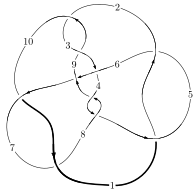
\includegraphics[width=112pt]{../../../GIT/diagram.site/Diagrams/png/195_10_111.png}\\
\ \ \ A knot diagram\footnotemark}&
\allowdisplaybreaks
\textbf{Linearized knot diagam} \\
\cline{2-2}
 &
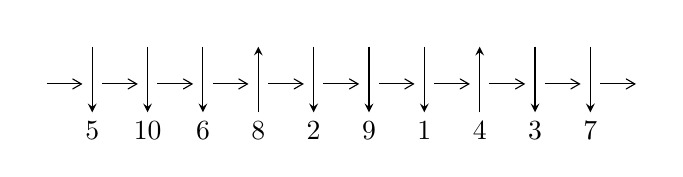
\begin{tikzpicture}[x=20pt, y=17pt]
	% nodes
	\node (C0) at (0, 0) {};
	\node (C1) at (1, 0) {};
	\node (C1U) at (1, +1) {};
	\node (C1D) at (1, -1) {5};

	\node (C2) at (2, 0) {};
	\node (C2U) at (2, +1) {};
	\node (C2D) at (2, -1) {10};

	\node (C3) at (3, 0) {};
	\node (C3U) at (3, +1) {};
	\node (C3D) at (3, -1) {6};

	\node (C4) at (4, 0) {};
	\node (C4U) at (4, +1) {};
	\node (C4D) at (4, -1) {8};

	\node (C5) at (5, 0) {};
	\node (C5U) at (5, +1) {};
	\node (C5D) at (5, -1) {2};

	\node (C6) at (6, 0) {};
	\node (C6U) at (6, +1) {};
	\node (C6D) at (6, -1) {9};

	\node (C7) at (7, 0) {};
	\node (C7U) at (7, +1) {};
	\node (C7D) at (7, -1) {1};

	\node (C8) at (8, 0) {};
	\node (C8U) at (8, +1) {};
	\node (C8D) at (8, -1) {4};

	\node (C9) at (9, 0) {};
	\node (C9U) at (9, +1) {};
	\node (C9D) at (9, -1) {3};

	\node (C10) at (10, 0) {};
	\node (C10U) at (10, +1) {};
	\node (C10D) at (10, -1) {7};
	\node (C11) at (11, 0) {};

	% arrows
	\draw[->,>={angle 60}]
	(C0) edge (C1) (C1) edge (C2) (C2) edge (C3) (C3) edge (C4) (C4) edge (C5) (C5) edge (C6) (C6) edge (C7) (C7) edge (C8) (C8) edge (C9) (C9) edge (C10) (C10) edge (C11) ;	\draw[->,>=stealth]
	(C1U) edge (C1D) (C2U) edge (C2D) (C3U) edge (C3D) (C4D) edge (C4U) (C5U) edge (C5D) (C6U) edge (C6D) (C7U) edge (C7D) (C8D) edge (C8U) (C9U) edge (C9D) (C10U) edge (C10D) ;
	\end{tikzpicture} \\
\hhline{~~} \\& 
\textbf{Solving Sequence} \\ \cline{2-2} 
 &
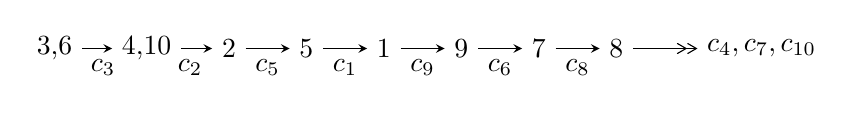
\begin{tikzpicture}[x=28pt, y=7pt]
	% node
	\node (A0) at (-1/8, 0) {3,6};
	\node (A1) at (17/16, 0) {4,10};
	\node (A2) at (17/8, 0) {2};
	\node (A3) at (25/8, 0) {5};
	\node (A4) at (33/8, 0) {1};
	\node (A5) at (41/8, 0) {9};
	\node (A6) at (49/8, 0) {7};
	\node (A7) at (57/8, 0) {8};
	\node (C1) at (1/2, -1) {$c_{3}$};
	\node (C2) at (13/8, -1) {$c_{2}$};
	\node (C3) at (21/8, -1) {$c_{5}$};
	\node (C4) at (29/8, -1) {$c_{1}$};
	\node (C5) at (37/8, -1) {$c_{9}$};
	\node (C6) at (45/8, -1) {$c_{6}$};
	\node (C7) at (53/8, -1) {$c_{8}$};
	\node (A8) at (9, 0) {$c_{4},c_{7},c_{10}$};

	% edge
	\draw[->,>=stealth]	
	(A0) edge (A1) (A1) edge (A2) (A2) edge (A3) (A3) edge (A4) (A4) edge (A5) (A5) edge (A6) (A6) edge (A7) ;
	\draw[->>,>={angle 60}]	
	(A7) edge (A8);
\end{tikzpicture} \\ 

\end{tabular} \\

\footnotetext{
The image of knot diagram is generated by the software ``\textbf{Draw programme}" developed by Andrew Bartholomew(\url{http://www.layer8.co.uk/maths/draw/index.htm\#Running-draw}), where we modified some parts for our purpose(\url{https://github.com/CATsTAILs/LinksPainter}).
}\phantom \\ \newline 
\centering \textbf{Ideals for irreducible components\footnotemark of $X_{\text{par}}$} 
 
\begin{align*}
I^u_{1}&=\langle 
39480 u^{13}-1274 u^{12}+\cdots+154933 b-318297,\;-39480 u^{13}+1274 u^{12}+\cdots+154933 a+163364,\\
\phantom{I^u_{1}}&\phantom{= \langle  }u^{14}+u^{13}+u^{12}+u^{11}+9 u^{10}+5 u^9+5 u^8+5 u^7+17 u^6+5 u^5+7 u^4-4 u^3+8 u^2- u+1\rangle \\
I^u_{2}&=\langle 
-8.27934\times10^{37} u^{29}-3.87934\times10^{38} u^{28}+\cdots+1.76638\times10^{35} b+2.60429\times10^{38},\\
\phantom{I^u_{2}}&\phantom{= \langle  }-2.70329\times10^{43} u^{29}-1.27006\times10^{44} u^{28}+\cdots+1.82589\times10^{40} a+8.84680\times10^{43},\\
\phantom{I^u_{2}}&\phantom{= \langle  }u^{30}+5 u^{29}+\cdots-14 u-1\rangle \\
I^u_{3}&=\langle 
4 u^5-2 u^4- u^3+b+16 u-8,\;-4 u^5+2 u^4+u^3+a-16 u+9,\;u^6- u^5+4 u^2-4 u+1\rangle \\
\\
\end{align*}
\raggedright * 3 irreducible components of $\dim_{\mathbb{C}}=0$, with total 50 representations.\\
\footnotetext{All coefficients of polynomials are rational numbers. But the coefficients are sometimes approximated in decimal forms when there is not enough margin.}
\newpage
\renewcommand{\arraystretch}{1}
\centering \section*{I. $I^u_{1}= \langle 39480 u^{13}-1274 u^{12}+\cdots+154933 b-318297,\;-3.95\times10^{4} u^{13}+1274 u^{12}+\cdots+1.55\times10^{5} a+1.63\times10^{5},\;u^{14}+u^{13}+\cdots- u+1 \rangle$}
\flushleft \textbf{(i) Arc colorings}\\
\begin{tabular}{m{7pt} m{180pt} m{7pt} m{180pt} }
\flushright $a_{3}=$&$\begin{pmatrix}1\\0\end{pmatrix}$ \\
\flushright $a_{6}=$&$\begin{pmatrix}0\\u\end{pmatrix}$ \\
\flushright $a_{4}=$&$\begin{pmatrix}1\\u^2\end{pmatrix}$ \\
\flushright $a_{10}=$&$\begin{pmatrix}0.254820 u^{13}-0.00822291 u^{12}+\cdots+3.57261 u-1.05442\\-0.254820 u^{13}+0.00822291 u^{12}+\cdots-3.57261 u+2.05442\end{pmatrix}$ \\
\flushright $a_{2}=$&$\begin{pmatrix}-1.23639 u^{13}-1.16081 u^{12}+\cdots-8.80020 u+1.50958\\1.49121 u^{13}+1.15259 u^{12}+\cdots+12.3728 u-2.56399\end{pmatrix}$ \\
\flushright $a_{5}=$&$\begin{pmatrix}-1.23092 u^{13}-1.01347 u^{12}+\cdots-9.83592 u+2.03566\\1.69744 u^{13}+1.28920 u^{12}+\cdots+14.8569 u-3.30753\end{pmatrix}$ \\
\flushright $a_{1}=$&$\begin{pmatrix}0.116528 u^{13}-0.0612071 u^{12}+\cdots+2.26064 u-0.978836\\-0.445618 u^{13}-0.321436 u^{12}+\cdots-4.37795 u+1.58789\end{pmatrix}$ \\
\flushright $a_{9}=$&$\begin{pmatrix}1\\-0.254820 u^{13}+0.00822291 u^{12}+\cdots-3.57261 u+2.05442\end{pmatrix}$ \\
\flushright $a_{7}=$&$\begin{pmatrix}- u\\-0.263043 u^{13}-0.260306 u^{12}+\cdots-0.799597 u-0.254820\end{pmatrix}$ \\
\flushright $a_{8}=$&$\begin{pmatrix}0.254820 u^{13}-0.00822291 u^{12}+\cdots+3.57261 u-1.05442\\-0.252083 u^{13}+0.0818935 u^{12}+\cdots-4.09047 u+2.31746\end{pmatrix}$\\&\end{tabular}
\flushleft \textbf{(ii) Obstruction class $= -1$}\\~\\
\flushleft \textbf{(iii) Cusp Shapes $= \frac{319153}{154933} u^{13}+\frac{874852}{154933} u^{12}+\cdots+\frac{171234}{154933} u+\frac{3427848}{154933}$}\\~\\
\newpage\renewcommand{\arraystretch}{1}
\flushleft \textbf{(iv) u-Polynomials at the component}\newline \\
\begin{tabular}{m{50pt}|m{274pt}}
Crossings & \hspace{64pt}u-Polynomials at each crossing \\
\hline $$\begin{aligned}c_{1},c_{5},c_{7}\\c_{10}\end{aligned}$$&$\begin{aligned}
&u^{14}-6 u^{12}+15 u^{10}- u^9-15 u^8+2 u^7+3 u^6- u^3+4 u^2+2 u+1
\end{aligned}$\\
\hline $$\begin{aligned}c_{2},c_{9}\end{aligned}$$&$\begin{aligned}
&u^{14}-10 u^{13}+\cdots-60 u+8
\end{aligned}$\\
\hline $$\begin{aligned}c_{3},c_{6}\end{aligned}$$&$\begin{aligned}
&u^{14}- u^{13}+\cdots+u+1
\end{aligned}$\\
\hline $$\begin{aligned}c_{4},c_{8}\end{aligned}$$&$\begin{aligned}
&u^{14}-11 u^{13}+\cdots-224 u+32
\end{aligned}$\\
\hline
\end{tabular}\\~\\
\newpage\renewcommand{\arraystretch}{1}
\flushleft \textbf{(v) Riley Polynomials at the component}\newline \\
\begin{tabular}{m{50pt}|m{274pt}}
Crossings & \hspace{64pt}Riley Polynomials at each crossing \\
\hline $$\begin{aligned}c_{1},c_{5},c_{7}\\c_{10}\end{aligned}$$&$\begin{aligned}
&y^{14}-12 y^{13}+\cdots+4 y+1
\end{aligned}$\\
\hline $$\begin{aligned}c_{2},c_{9}\end{aligned}$$&$\begin{aligned}
&y^{14}+4 y^{13}+\cdots+240 y+64
\end{aligned}$\\
\hline $$\begin{aligned}c_{3},c_{6}\end{aligned}$$&$\begin{aligned}
&y^{14}+y^{13}+\cdots+15 y+1
\end{aligned}$\\
\hline $$\begin{aligned}c_{4},c_{8}\end{aligned}$$&$\begin{aligned}
&y^{14}+5 y^{13}+\cdots+512 y+1024
\end{aligned}$\\
\hline
\end{tabular}\\~\\
\newpage\flushleft \textbf{(vi) Complex Volumes and Cusp Shapes}
$$\begin{array}{c|c|c}  
\text{Solutions to }I^u_{1}& \I (\text{vol} + \sqrt{-1}CS) & \text{Cusp shape}\\
 \hline 
\begin{aligned}
u &= -0.480433 + 0.861641 I \\
a &= \phantom{-}0.839666 + 1.114140 I \\
b &= \phantom{-}0.160334 - 1.114140 I\end{aligned}
 & \phantom{-}3.38735 - 0.25005 I & -0.72285 + 2.46287 I \\ \hline\begin{aligned}
u &= -0.480433 - 0.861641 I \\
a &= \phantom{-}0.839666 - 1.114140 I \\
b &= \phantom{-}0.160334 + 1.114140 I\end{aligned}
 & \phantom{-}3.38735 + 0.25005 I & -0.72285 - 2.46287 I \\ \hline\begin{aligned}
u &= -1.048940 + 0.652179 I \\
a &= -0.187430 - 0.232557 I \\
b &= \phantom{-}1.187430 + 0.232557 I\end{aligned}
 & -10.88730 + 7.87015 I & -12.80126 - 5.10311 I \\ \hline\begin{aligned}
u &= -1.048940 - 0.652179 I \\
a &= -0.187430 + 0.232557 I \\
b &= \phantom{-}1.187430 - 0.232557 I\end{aligned}
 & -10.88730 - 7.87015 I & -12.80126 + 5.10311 I \\ \hline\begin{aligned}
u &= \phantom{-}0.486006 + 0.497659 I \\
a &= \phantom{-}0.703941 + 0.328567 I \\
b &= \phantom{-}0.296059 - 0.328567 I\end{aligned}
 & -0.46723 - 1.34385 I & -4.53324 + 5.44435 I \\ \hline\begin{aligned}
u &= \phantom{-}0.486006 - 0.497659 I \\
a &= \phantom{-}0.703941 - 0.328567 I \\
b &= \phantom{-}0.296059 + 0.328567 I\end{aligned}
 & -0.46723 + 1.34385 I & -4.53324 - 5.44435 I \\ \hline\begin{aligned}
u &= \phantom{-}0.775295 + 1.049040 I \\
a &= \phantom{-}0.248822 - 1.259320 I \\
b &= \phantom{-}0.75118 + 1.25932 I\end{aligned}
 & -1.57595 - 8.21733 I & -8.00559 + 6.90533 I \\ \hline\begin{aligned}
u &= \phantom{-}0.775295 - 1.049040 I \\
a &= \phantom{-}0.248822 + 1.259320 I \\
b &= \phantom{-}0.75118 - 1.25932 I\end{aligned}
 & -1.57595 + 8.21733 I & -8.00559 - 6.90533 I \\ \hline\begin{aligned}
u &= \phantom{-}0.96587 + 1.05626 I \\
a &= \phantom{-}0.706527 - 1.007890 I \\
b &= \phantom{-}0.293473 + 1.007890 I\end{aligned}
 & \phantom{-}1.24241 - 4.01184 I & -4.00908 + 1.51637 I \\ \hline\begin{aligned}
u &= \phantom{-}0.96587 - 1.05626 I \\
a &= \phantom{-}0.706527 + 1.007890 I \\
b &= \phantom{-}0.293473 - 1.007890 I\end{aligned}
 & \phantom{-}1.24241 + 4.01184 I & -4.00908 - 1.51637 I\\
 \hline 
 \end{array}$$\newpage$$\begin{array}{c|c|c}  
\text{Solutions to }I^u_{1}& \I (\text{vol} + \sqrt{-1}CS) & \text{Cusp shape}\\
 \hline 
\begin{aligned}
u &= \phantom{-}0.025861 + 0.375115 I \\
a &= -0.66482 + 1.30083 I \\
b &= \phantom{-}1.66482 - 1.30083 I\end{aligned}
 & -3.88016 - 0.30866 I & \phantom{-}21.1851 - 1.2071 I \\ \hline\begin{aligned}
u &= \phantom{-}0.025861 - 0.375115 I \\
a &= -0.66482 - 1.30083 I \\
b &= \phantom{-}1.66482 + 1.30083 I\end{aligned}
 & -3.88016 + 0.30866 I & \phantom{-}21.1851 + 1.2071 I \\ \hline\begin{aligned}
u &= -1.22366 + 1.15195 I \\
a &= \phantom{-}0.353292 + 1.290880 I \\
b &= \phantom{-}0.64671 - 1.29088 I\end{aligned}
 & -7.5584 + 14.2650 I & -9.61306 - 7.45903 I \\ \hline\begin{aligned}
u &= -1.22366 - 1.15195 I \\
a &= \phantom{-}0.353292 - 1.290880 I \\
b &= \phantom{-}0.64671 + 1.29088 I\end{aligned}
 & -7.5584 - 14.2650 I & -9.61306 + 7.45903 I\\
 \hline 
 \end{array}$$\newpage\newpage\renewcommand{\arraystretch}{1}
\centering \section*{II. $I^u_{2}= \langle -8.28\times10^{37} u^{29}-3.88\times10^{38} u^{28}+\cdots+1.77\times10^{35} b+2.60\times10^{38},\;-2.70\times10^{43} u^{29}-1.27\times10^{44} u^{28}+\cdots+1.83\times10^{40} a+8.85\times10^{43},\;u^{30}+5 u^{29}+\cdots-14 u-1 \rangle$}
\flushleft \textbf{(i) Arc colorings}\\
\begin{tabular}{m{7pt} m{180pt} m{7pt} m{180pt} }
\flushright $a_{3}=$&$\begin{pmatrix}1\\0\end{pmatrix}$ \\
\flushright $a_{6}=$&$\begin{pmatrix}0\\u\end{pmatrix}$ \\
\flushright $a_{4}=$&$\begin{pmatrix}1\\u^2\end{pmatrix}$ \\
\flushright $a_{10}=$&$\begin{pmatrix}1480.53 u^{29}+6955.82 u^{28}+\cdots-52108.0 u-4845.20\\468.718 u^{29}+2196.21 u^{28}+\cdots-16062.1 u-1474.36\end{pmatrix}$ \\
\flushright $a_{2}=$&$\begin{pmatrix}-1085.37 u^{29}-5070.52 u^{28}+\cdots+36285.0 u+3322.75\\350.689 u^{29}+1665.42 u^{28}+\cdots-13806.5 u-1340.83\end{pmatrix}$ \\
\flushright $a_{5}=$&$\begin{pmatrix}-991.168 u^{29}-4565.91 u^{28}+\cdots+28334.6 u+2429.77\\398.530 u^{29}+1884.97 u^{28}+\cdots-15091.1 u-1445.96\end{pmatrix}$ \\
\flushright $a_{1}=$&$\begin{pmatrix}-1780.35 u^{29}-8495.89 u^{28}+\cdots+72515.7 u+7062.23\\-181.114 u^{29}-833.946 u^{28}+\cdots+5098.47 u+429.698\end{pmatrix}$ \\
\flushright $a_{9}=$&$\begin{pmatrix}1949.25 u^{29}+9152.03 u^{28}+\cdots-68170.1 u-6319.56\\468.718 u^{29}+2196.21 u^{28}+\cdots-16062.1 u-1474.36\end{pmatrix}$ \\
\flushright $a_{7}=$&$\begin{pmatrix}1388.04 u^{29}+6649.23 u^{28}+\cdots-58366.7 u-5729.66\\268.310 u^{29}+1245.03 u^{28}+\cdots-8303.63 u-734.682\end{pmatrix}$ \\
\flushright $a_{8}=$&$\begin{pmatrix}1659.04 u^{29}+7795.68 u^{28}+\cdots-58477.9 u-5439.43\\437.990 u^{29}+2052.51 u^{28}+\cdots-15026.1 u-1379.63\end{pmatrix}$\\&\end{tabular}
\flushleft \textbf{(ii) Obstruction class $= -1$}\\~\\
\flushleft \textbf{(iii) Cusp Shapes $= -1720.55 u^{29}-8153.31 u^{28}+\cdots+66031.6 u+6330.33$}\\~\\
\newpage\renewcommand{\arraystretch}{1}
\flushleft \textbf{(iv) u-Polynomials at the component}\newline \\
\begin{tabular}{m{50pt}|m{274pt}}
Crossings & \hspace{64pt}u-Polynomials at each crossing \\
\hline $$\begin{aligned}c_{1},c_{5},c_{7}\\c_{10}\end{aligned}$$&$\begin{aligned}
&u^{30}+u^{29}+\cdots+212 u+11
\end{aligned}$\\
\hline $$\begin{aligned}c_{2},c_{9}\end{aligned}$$&$\begin{aligned}
&(u^5+u^4+2 u^3+u^2+u+1)^6
\end{aligned}$\\
\hline $$\begin{aligned}c_{3},c_{6}\end{aligned}$$&$\begin{aligned}
&u^{30}-5 u^{29}+\cdots+14 u-1
\end{aligned}$\\
\hline $$\begin{aligned}c_{4},c_{8}\end{aligned}$$&$\begin{aligned}
&(u^3+u^2+2 u+1)^{10}
\end{aligned}$\\
\hline
\end{tabular}\\~\\
\newpage\renewcommand{\arraystretch}{1}
\flushleft \textbf{(v) Riley Polynomials at the component}\newline \\
\begin{tabular}{m{50pt}|m{274pt}}
Crossings & \hspace{64pt}Riley Polynomials at each crossing \\
\hline $$\begin{aligned}c_{1},c_{5},c_{7}\\c_{10}\end{aligned}$$&$\begin{aligned}
&y^{30}-25 y^{29}+\cdots-32360 y+121
\end{aligned}$\\
\hline $$\begin{aligned}c_{2},c_{9}\end{aligned}$$&$\begin{aligned}
&(y^5+3 y^4+4 y^3+y^2- y-1)^6
\end{aligned}$\\
\hline $$\begin{aligned}c_{3},c_{6}\end{aligned}$$&$\begin{aligned}
&y^{30}-5 y^{29}+\cdots-56 y+1
\end{aligned}$\\
\hline $$\begin{aligned}c_{4},c_{8}\end{aligned}$$&$\begin{aligned}
&(y^3+3 y^2+2 y-1)^{10}
\end{aligned}$\\
\hline
\end{tabular}\\~\\
\newpage\flushleft \textbf{(vi) Complex Volumes and Cusp Shapes}
$$\begin{array}{c|c|c}  
\text{Solutions to }I^u_{2}& \I (\text{vol} + \sqrt{-1}CS) & \text{Cusp shape}\\
 \hline 
\begin{aligned}
u &= -0.711013 + 0.598106 I \\
a &= -0.891374 - 0.831846 I \\
b &= -0.455697 + 1.200150 I\end{aligned}
 & \phantom{-}2.05122 + 4.40083 I & -2.23618 - 3.49859 I \\ \hline\begin{aligned}
u &= -0.711013 - 0.598106 I \\
a &= -0.891374 + 0.831846 I \\
b &= -0.455697 - 1.200150 I\end{aligned}
 & \phantom{-}2.05122 - 4.40083 I & -2.23618 + 3.49859 I \\ \hline\begin{aligned}
u &= -1.108120 + 0.043065 I \\
a &= \phantom{-}0.244564 - 0.869058 I \\
b &= \phantom{-}0.339110 - 0.822375 I\end{aligned}
 & -7.62983 - 1.29754 I & -12.99464 - 1.45120 I \\ \hline\begin{aligned}
u &= -1.108120 - 0.043065 I \\
a &= \phantom{-}0.244564 + 0.869058 I \\
b &= \phantom{-}0.339110 + 0.822375 I\end{aligned}
 & -7.62983 + 1.29754 I & -12.99464 + 1.45120 I \\ \hline\begin{aligned}
u &= \phantom{-}0.750590 + 0.816532 I \\
a &= -0.254359 + 0.536218 I \\
b &= -0.766826\phantom{ +0.000000I}\end{aligned}
 & -5.55785 - 2.82812 I & -12.02861 + 2.97945 I \\ \hline\begin{aligned}
u &= \phantom{-}0.750590 - 0.816532 I \\
a &= -0.254359 - 0.536218 I \\
b &= -0.766826\phantom{ +0.000000I}\end{aligned}
 & -5.55785 + 2.82812 I & -12.02861 - 2.97945 I \\ \hline\begin{aligned}
u &= \phantom{-}0.723473 + 0.513234 I \\
a &= \phantom{-}0.226305 - 0.956455 I \\
b &= -0.455697 + 1.200150 I\end{aligned}
 & -2.08637 + 1.57271 I & -8.76544 - 0.51914 I \\ \hline\begin{aligned}
u &= \phantom{-}0.723473 - 0.513234 I \\
a &= \phantom{-}0.226305 + 0.956455 I \\
b &= -0.455697 - 1.200150 I\end{aligned}
 & -2.08637 - 1.57271 I & -8.76544 + 0.51914 I \\ \hline\begin{aligned}
u &= \phantom{-}0.375132 + 0.793055 I \\
a &= -0.26221 - 2.41312 I \\
b &= \phantom{-}0.339110 + 0.822375 I\end{aligned}
 & -3.49225 - 1.53058 I & -6.46537 + 4.43065 I \\ \hline\begin{aligned}
u &= \phantom{-}0.375132 - 0.793055 I \\
a &= -0.26221 + 2.41312 I \\
b &= \phantom{-}0.339110 - 0.822375 I\end{aligned}
 & -3.49225 + 1.53058 I & -6.46537 - 4.43065 I\\
 \hline 
 \end{array}$$\newpage$$\begin{array}{c|c|c}  
\text{Solutions to }I^u_{2}& \I (\text{vol} + \sqrt{-1}CS) & \text{Cusp shape}\\
 \hline 
\begin{aligned}
u &= \phantom{-}0.953025 + 0.838377 I \\
a &= -1.10687 + 1.14990 I \\
b &= -0.455697 - 1.200150 I\end{aligned}
 & -2.08637 - 7.22895 I & \phantom{-0.000000 } 0 \\ \hline\begin{aligned}
u &= \phantom{-}0.953025 - 0.838377 I \\
a &= -1.10687 - 1.14990 I \\
b &= -0.455697 + 1.200150 I\end{aligned}
 & -2.08637 + 7.22895 I & \phantom{-0.000000 } 0 \\ \hline\begin{aligned}
u &= -1.204330 + 0.431350 I \\
a &= -0.000782 + 0.403066 I \\
b &= -0.766826\phantom{ +0.000000I}\end{aligned}
 & -5.55785 + 2.82812 I & \phantom{-0.000000 } 0 \\ \hline\begin{aligned}
u &= -1.204330 - 0.431350 I \\
a &= -0.000782 - 0.403066 I \\
b &= -0.766826\phantom{ +0.000000I}\end{aligned}
 & -5.55785 - 2.82812 I & \phantom{-0.000000 } 0 \\ \hline\begin{aligned}
u &= \phantom{-}0.737499 + 1.067560 I \\
a &= -0.235020 + 1.389000 I \\
b &= -0.455697 - 1.200150 I\end{aligned}
 & \phantom{-}2.05122 - 4.40083 I & \phantom{-0.000000 } 0 \\ \hline\begin{aligned}
u &= \phantom{-}0.737499 - 1.067560 I \\
a &= -0.235020 - 1.389000 I \\
b &= -0.455697 + 1.200150 I\end{aligned}
 & \phantom{-}2.05122 + 4.40083 I & \phantom{-0.000000 } 0 \\ \hline\begin{aligned}
u &= \phantom{-}0.680032\phantom{ +0.000000I} \\
a &= \phantom{-}0.340860\phantom{ +0.000000I} \\
b &= -0.766826\phantom{ +0.000000I}\end{aligned}
 & -1.42027\phantom{ +0.000000I} & -5.49930\phantom{ +0.000000I} \\ \hline\begin{aligned}
u &= \phantom{-}1.290400 + 0.535753 I \\
a &= -0.308791 + 0.195205 I \\
b &= \phantom{-}0.339110 - 0.822375 I\end{aligned}
 & -3.49225 + 1.53058 I & \phantom{-0.000000 } 0 \\ \hline\begin{aligned}
u &= \phantom{-}1.290400 - 0.535753 I \\
a &= -0.308791 - 0.195205 I \\
b &= \phantom{-}0.339110 + 0.822375 I\end{aligned}
 & -3.49225 - 1.53058 I & \phantom{-0.000000 } 0 \\ \hline\begin{aligned}
u &= -0.320748 + 0.034597 I \\
a &= \phantom{-}5.85652 - 4.23753 I \\
b &= \phantom{-}0.339110 + 0.822375 I\end{aligned}
 & -7.62983 - 4.35870 I & -12.9946 + 7.4101 I\\
 \hline 
 \end{array}$$\newpage$$\begin{array}{c|c|c}  
\text{Solutions to }I^u_{2}& \I (\text{vol} + \sqrt{-1}CS) & \text{Cusp shape}\\
 \hline 
\begin{aligned}
u &= -0.320748 - 0.034597 I \\
a &= \phantom{-}5.85652 + 4.23753 I \\
b &= \phantom{-}0.339110 - 0.822375 I\end{aligned}
 & -7.62983 + 4.35870 I & -12.9946 - 7.4101 I \\ \hline\begin{aligned}
u &= -0.291032 + 0.058576 I \\
a &= -1.59228 - 3.37585 I \\
b &= -0.455697 + 1.200150 I\end{aligned}
 & -2.08637 + 1.57271 I & -8.76544 - 0.51914 I \\ \hline\begin{aligned}
u &= -0.291032 - 0.058576 I \\
a &= -1.59228 + 3.37585 I \\
b &= -0.455697 - 1.200150 I\end{aligned}
 & -2.08637 - 1.57271 I & -8.76544 + 0.51914 I \\ \hline\begin{aligned}
u &= -0.289671\phantom{ +0.000000I} \\
a &= -1.58078\phantom{ +0.000000I} \\
b &= -0.766826\phantom{ +0.000000I}\end{aligned}
 & -1.42027\phantom{ +0.000000I} & -5.49930\phantom{ +0.000000I} \\ \hline\begin{aligned}
u &= -0.57394 + 1.89944 I \\
a &= -0.156804 + 1.350680 I \\
b &= \phantom{-}0.339110 - 0.822375 I\end{aligned}
 & -7.62983 - 1.29754 I & \phantom{-0.000000 } 0 \\ \hline\begin{aligned}
u &= -0.57394 - 1.89944 I \\
a &= -0.156804 - 1.350680 I \\
b &= \phantom{-}0.339110 + 0.822375 I\end{aligned}
 & -7.62983 + 1.29754 I & \phantom{-0.000000 } 0 \\ \hline\begin{aligned}
u &= -1.44704 + 1.35792 I \\
a &= -0.183612 - 1.220710 I \\
b &= -0.455697 + 1.200150 I\end{aligned}
 & -2.08637 + 7.22895 I & \phantom{-0.000000 } 0 \\ \hline\begin{aligned}
u &= -1.44704 - 1.35792 I \\
a &= -0.183612 + 1.220710 I \\
b &= -0.455697 - 1.200150 I\end{aligned}
 & -2.08637 - 7.22895 I & \phantom{-0.000000 } 0 \\ \hline\begin{aligned}
u &= -1.86908 + 1.30976 I \\
a &= -0.215319 - 0.754139 I \\
b &= \phantom{-}0.339110 + 0.822375 I\end{aligned}
 & -7.62983 - 4.35870 I & \phantom{-0.000000 } 0 \\ \hline\begin{aligned}
u &= -1.86908 - 1.30976 I \\
a &= -0.215319 + 0.754139 I \\
b &= \phantom{-}0.339110 - 0.822375 I\end{aligned}
 & -7.62983 + 4.35870 I & \phantom{-0.000000 } 0\\
 \hline 
 \end{array}$$\newpage\newpage\renewcommand{\arraystretch}{1}
\centering \section*{III. $I^u_{3}= \langle 4 u^5-2 u^4- u^3+b+16 u-8,\;-4 u^5+2 u^4+u^3+a-16 u+9,\;u^6- u^5+4 u^2-4 u+1 \rangle$}
\flushleft \textbf{(i) Arc colorings}\\
\begin{tabular}{m{7pt} m{180pt} m{7pt} m{180pt} }
\flushright $a_{3}=$&$\begin{pmatrix}1\\0\end{pmatrix}$ \\
\flushright $a_{6}=$&$\begin{pmatrix}0\\u\end{pmatrix}$ \\
\flushright $a_{4}=$&$\begin{pmatrix}1\\u^2\end{pmatrix}$ \\
\flushright $a_{10}=$&$\begin{pmatrix}4 u^5-2 u^4- u^3+16 u-9\\-4 u^5+2 u^4+u^3-16 u+8\end{pmatrix}$ \\
\flushright $a_{2}=$&$\begin{pmatrix}-3 u^5+2 u^4+u^3-12 u+8\\- u^5-4 u+1\end{pmatrix}$ \\
\flushright $a_{5}=$&$\begin{pmatrix}-5 u^5+3 u^4+u^3+u^2-20 u+12\\u-1\end{pmatrix}$ \\
\flushright $a_{1}=$&$\begin{pmatrix}4 u^5-2 u^4- u^3+15 u-8\\-2 u^5+u^4-7 u+3\end{pmatrix}$ \\
\flushright $a_{9}=$&$\begin{pmatrix}-1\\-4 u^5+2 u^4+u^3-16 u+8\end{pmatrix}$ \\
\flushright $a_{7}=$&$\begin{pmatrix}- u\\-2 u^5+u^4-7 u+4\end{pmatrix}$ \\
\flushright $a_{8}=$&$\begin{pmatrix}4 u^5-2 u^4- u^3- u^2+16 u-9\\-3 u^5+u^4+u^3-12 u+6\end{pmatrix}$\\&\end{tabular}
\flushleft \textbf{(ii) Obstruction class $= 1$}\\~\\
\flushleft \textbf{(iii) Cusp Shapes $= -25 u^5+10 u^4+7 u^3+5 u^2-96 u+32$}\\~\\
\newpage\renewcommand{\arraystretch}{1}
\flushleft \textbf{(iv) u-Polynomials at the component}\newline \\
\begin{tabular}{m{50pt}|m{274pt}}
Crossings & \hspace{64pt}u-Polynomials at each crossing \\
\hline $$\begin{aligned}c_{1},c_{7}\end{aligned}$$&$\begin{aligned}
&u^6+2 u^5- u^4-4 u^3- u^2+u+1
\end{aligned}$\\
\hline $$\begin{aligned}c_{2}\end{aligned}$$&$\begin{aligned}
&u^6+u^5+u^4- u^2-1
\end{aligned}$\\
\hline $$\begin{aligned}c_{3},c_{6}\end{aligned}$$&$\begin{aligned}
&u^6- u^5+4 u^2-4 u+1
\end{aligned}$\\
\hline $$\begin{aligned}c_{4}\end{aligned}$$&$\begin{aligned}
&u^6+u^4- u^2- u-1
\end{aligned}$\\
\hline $$\begin{aligned}c_{5},c_{10}\end{aligned}$$&$\begin{aligned}
&u^6-2 u^5- u^4+4 u^3- u^2- u+1
\end{aligned}$\\
\hline $$\begin{aligned}c_{8}\end{aligned}$$&$\begin{aligned}
&u^6+u^4- u^2+u-1
\end{aligned}$\\
\hline $$\begin{aligned}c_{9}\end{aligned}$$&$\begin{aligned}
&u^6- u^5+u^4- u^2-1
\end{aligned}$\\
\hline
\end{tabular}\\~\\
\newpage\renewcommand{\arraystretch}{1}
\flushleft \textbf{(v) Riley Polynomials at the component}\newline \\
\begin{tabular}{m{50pt}|m{274pt}}
Crossings & \hspace{64pt}Riley Polynomials at each crossing \\
\hline $$\begin{aligned}c_{1},c_{5},c_{7}\\c_{10}\end{aligned}$$&$\begin{aligned}
&y^6-6 y^5+15 y^4-16 y^3+7 y^2-3 y+1
\end{aligned}$\\
\hline $$\begin{aligned}c_{2},c_{9}\end{aligned}$$&$\begin{aligned}
&y^6+y^5- y^4-4 y^3- y^2+2 y+1
\end{aligned}$\\
\hline $$\begin{aligned}c_{3},c_{6}\end{aligned}$$&$\begin{aligned}
&y^6- y^5+8 y^4-6 y^3+16 y^2-8 y+1
\end{aligned}$\\
\hline $$\begin{aligned}c_{4},c_{8}\end{aligned}$$&$\begin{aligned}
&y^6+2 y^5- y^4-4 y^3- y^2+y+1
\end{aligned}$\\
\hline
\end{tabular}\\~\\
\newpage\flushleft \textbf{(vi) Complex Volumes and Cusp Shapes}
$$\begin{array}{c|c|c}  
\text{Solutions to }I^u_{3}& \I (\text{vol} + \sqrt{-1}CS) & \text{Cusp shape}\\
 \hline 
\begin{aligned}
u &= \phantom{-}1.008100 + 0.927438 I \\
a &= -0.516513 + 1.114980 I \\
b &= -0.483487 - 1.114980 I\end{aligned}
 & \phantom{-}0.45357 - 5.18068 I & -8.71093 + 6.15331 I \\ \hline\begin{aligned}
u &= \phantom{-}1.008100 - 0.927438 I \\
a &= -0.516513 - 1.114980 I \\
b &= -0.483487 + 1.114980 I\end{aligned}
 & \phantom{-}0.45357 + 5.18068 I & -8.71093 - 6.15331 I \\ \hline\begin{aligned}
u &= \phantom{-}0.584070\phantom{ +0.000000I} \\
a &= \phantom{-}0.185012\phantom{ +0.000000I} \\
b &= -1.18501\phantom{ +0.000000I}\end{aligned}
 & -2.13209\phantom{ +0.000000I} & -21.5060\phantom{ +0.000000I} \\ \hline\begin{aligned}
u &= -1.02499 + 0.98915 I \\
a &= -1.124000 - 0.785288 I \\
b &= \phantom{-}0.124001 + 0.785288 I\end{aligned}
 & -7.16447 - 3.17324 I & -9.24905 + 1.07022 I \\ \hline\begin{aligned}
u &= -1.02499 - 0.98915 I \\
a &= -1.124000 + 0.785288 I \\
b &= \phantom{-}0.124001 - 0.785288 I\end{aligned}
 & -7.16447 + 3.17324 I & -9.24905 - 1.07022 I \\ \hline\begin{aligned}
u &= \phantom{-}0.449699\phantom{ +0.000000I} \\
a &= -1.90398\phantom{ +0.000000I} \\
b &= \phantom{-}0.903984\phantom{ +0.000000I}\end{aligned}
 & -4.18532\phantom{ +0.000000I} & -9.57420\phantom{ +0.000000I}\\
 \hline 
 \end{array}$$\newpage
\newpage\renewcommand{\arraystretch}{1}
\centering \section*{ IV. u-Polynomials}
\begin{tabular}{m{50pt}|m{274pt}}
Crossings & \hspace{64pt}u-Polynomials at each crossing \\
\hline $$\begin{aligned}c_{1},c_{7}\end{aligned}$$&$\begin{aligned}
&(u^6+2 u^5- u^4-4 u^3- u^2+u+1)\\
&\cdot(u^{14}-6 u^{12}+15 u^{10}- u^9-15 u^8+2 u^7+3 u^6- u^3+4 u^2+2 u+1)\\
&\cdot(u^{30}+u^{29}+\cdots+212 u+11)
\end{aligned}$\\
\hline $$\begin{aligned}c_{2}\end{aligned}$$&$\begin{aligned}
&(u^5+u^4+2 u^3+u^2+u+1)^6(u^6+u^5+u^4- u^2-1)\\
&\cdot(u^{14}-10 u^{13}+\cdots-60 u+8)
\end{aligned}$\\
\hline $$\begin{aligned}c_{3},c_{6}\end{aligned}$$&$\begin{aligned}
&(u^6- u^5+4 u^2-4 u+1)(u^{14}- u^{13}+\cdots+u+1)\\
&\cdot(u^{30}-5 u^{29}+\cdots+14 u-1)
\end{aligned}$\\
\hline $$\begin{aligned}c_{4}\end{aligned}$$&$\begin{aligned}
&(u^3+u^2+2 u+1)^{10}(u^6+u^4- u^2- u-1)\\
&\cdot(u^{14}-11 u^{13}+\cdots-224 u+32)
\end{aligned}$\\
\hline $$\begin{aligned}c_{5},c_{10}\end{aligned}$$&$\begin{aligned}
&(u^6-2 u^5- u^4+4 u^3- u^2- u+1)\\
&\cdot(u^{14}-6 u^{12}+15 u^{10}- u^9-15 u^8+2 u^7+3 u^6- u^3+4 u^2+2 u+1)\\
&\cdot(u^{30}+u^{29}+\cdots+212 u+11)
\end{aligned}$\\
\hline $$\begin{aligned}c_{8}\end{aligned}$$&$\begin{aligned}
&(u^3+u^2+2 u+1)^{10}(u^6+u^4- u^2+u-1)\\
&\cdot(u^{14}-11 u^{13}+\cdots-224 u+32)
\end{aligned}$\\
\hline $$\begin{aligned}c_{9}\end{aligned}$$&$\begin{aligned}
&(u^5+u^4+2 u^3+u^2+u+1)^6(u^6- u^5+u^4- u^2-1)\\
&\cdot(u^{14}-10 u^{13}+\cdots-60 u+8)
\end{aligned}$\\
\hline
\end{tabular}\newpage\renewcommand{\arraystretch}{1}
\centering \section*{ V. Riley Polynomials}
\begin{tabular}{m{50pt}|m{274pt}}
Crossings & \hspace{64pt}Riley Polynomials at each crossing \\
\hline $$\begin{aligned}c_{1},c_{5},c_{7}\\c_{10}\end{aligned}$$&$\begin{aligned}
&(y^6-6 y^5+\cdots-3 y+1)(y^{14}-12 y^{13}+\cdots+4 y+1)\\
&\cdot(y^{30}-25 y^{29}+\cdots-32360 y+121)
\end{aligned}$\\
\hline $$\begin{aligned}c_{2},c_{9}\end{aligned}$$&$\begin{aligned}
&(y^5+3 y^4+4 y^3+y^2- y-1)^6(y^6+y^5- y^4-4 y^3- y^2+2 y+1)\\
&\cdot(y^{14}+4 y^{13}+\cdots+240 y+64)
\end{aligned}$\\
\hline $$\begin{aligned}c_{3},c_{6}\end{aligned}$$&$\begin{aligned}
&(y^6- y^5+\cdots-8 y+1)(y^{14}+y^{13}+\cdots+15 y+1)\\
&\cdot(y^{30}-5 y^{29}+\cdots-56 y+1)
\end{aligned}$\\
\hline $$\begin{aligned}c_{4},c_{8}\end{aligned}$$&$\begin{aligned}
&(y^3+3 y^2+2 y-1)^{10}(y^6+2 y^5- y^4-4 y^3- y^2+y+1)\\
&\cdot(y^{14}+5 y^{13}+\cdots+512 y+1024)
\end{aligned}$\\
\hline
\end{tabular}
\vskip 2pc
\end{document}